% Options for packages loaded elsewhere
\PassOptionsToPackage{unicode}{hyperref}
\PassOptionsToPackage{hyphens}{url}
\PassOptionsToPackage{dvipsnames,svgnames,x11names}{xcolor}
%
\documentclass[
  letterpaper,
  DIV=11,
  numbers=noendperiod]{scrreprt}

\usepackage{amsmath,amssymb}
\usepackage{iftex}
\ifPDFTeX
  \usepackage[T1]{fontenc}
  \usepackage[utf8]{inputenc}
  \usepackage{textcomp} % provide euro and other symbols
\else % if luatex or xetex
  \usepackage{unicode-math}
  \defaultfontfeatures{Scale=MatchLowercase}
  \defaultfontfeatures[\rmfamily]{Ligatures=TeX,Scale=1}
\fi
\usepackage{lmodern}
\ifPDFTeX\else  
    % xetex/luatex font selection
\fi
% Use upquote if available, for straight quotes in verbatim environments
\IfFileExists{upquote.sty}{\usepackage{upquote}}{}
\IfFileExists{microtype.sty}{% use microtype if available
  \usepackage[]{microtype}
  \UseMicrotypeSet[protrusion]{basicmath} % disable protrusion for tt fonts
}{}
\makeatletter
\@ifundefined{KOMAClassName}{% if non-KOMA class
  \IfFileExists{parskip.sty}{%
    \usepackage{parskip}
  }{% else
    \setlength{\parindent}{0pt}
    \setlength{\parskip}{6pt plus 2pt minus 1pt}}
}{% if KOMA class
  \KOMAoptions{parskip=half}}
\makeatother
\usepackage{xcolor}
\setlength{\emergencystretch}{3em} % prevent overfull lines
\setcounter{secnumdepth}{5}
% Make \paragraph and \subparagraph free-standing
\ifx\paragraph\undefined\else
  \let\oldparagraph\paragraph
  \renewcommand{\paragraph}[1]{\oldparagraph{#1}\mbox{}}
\fi
\ifx\subparagraph\undefined\else
  \let\oldsubparagraph\subparagraph
  \renewcommand{\subparagraph}[1]{\oldsubparagraph{#1}\mbox{}}
\fi

\usepackage{color}
\usepackage{fancyvrb}
\newcommand{\VerbBar}{|}
\newcommand{\VERB}{\Verb[commandchars=\\\{\}]}
\DefineVerbatimEnvironment{Highlighting}{Verbatim}{commandchars=\\\{\}}
% Add ',fontsize=\small' for more characters per line
\usepackage{framed}
\definecolor{shadecolor}{RGB}{241,243,245}
\newenvironment{Shaded}{\begin{snugshade}}{\end{snugshade}}
\newcommand{\AlertTok}[1]{\textcolor[rgb]{0.68,0.00,0.00}{#1}}
\newcommand{\AnnotationTok}[1]{\textcolor[rgb]{0.37,0.37,0.37}{#1}}
\newcommand{\AttributeTok}[1]{\textcolor[rgb]{0.40,0.45,0.13}{#1}}
\newcommand{\BaseNTok}[1]{\textcolor[rgb]{0.68,0.00,0.00}{#1}}
\newcommand{\BuiltInTok}[1]{\textcolor[rgb]{0.00,0.23,0.31}{#1}}
\newcommand{\CharTok}[1]{\textcolor[rgb]{0.13,0.47,0.30}{#1}}
\newcommand{\CommentTok}[1]{\textcolor[rgb]{0.37,0.37,0.37}{#1}}
\newcommand{\CommentVarTok}[1]{\textcolor[rgb]{0.37,0.37,0.37}{\textit{#1}}}
\newcommand{\ConstantTok}[1]{\textcolor[rgb]{0.56,0.35,0.01}{#1}}
\newcommand{\ControlFlowTok}[1]{\textcolor[rgb]{0.00,0.23,0.31}{#1}}
\newcommand{\DataTypeTok}[1]{\textcolor[rgb]{0.68,0.00,0.00}{#1}}
\newcommand{\DecValTok}[1]{\textcolor[rgb]{0.68,0.00,0.00}{#1}}
\newcommand{\DocumentationTok}[1]{\textcolor[rgb]{0.37,0.37,0.37}{\textit{#1}}}
\newcommand{\ErrorTok}[1]{\textcolor[rgb]{0.68,0.00,0.00}{#1}}
\newcommand{\ExtensionTok}[1]{\textcolor[rgb]{0.00,0.23,0.31}{#1}}
\newcommand{\FloatTok}[1]{\textcolor[rgb]{0.68,0.00,0.00}{#1}}
\newcommand{\FunctionTok}[1]{\textcolor[rgb]{0.28,0.35,0.67}{#1}}
\newcommand{\ImportTok}[1]{\textcolor[rgb]{0.00,0.46,0.62}{#1}}
\newcommand{\InformationTok}[1]{\textcolor[rgb]{0.37,0.37,0.37}{#1}}
\newcommand{\KeywordTok}[1]{\textcolor[rgb]{0.00,0.23,0.31}{#1}}
\newcommand{\NormalTok}[1]{\textcolor[rgb]{0.00,0.23,0.31}{#1}}
\newcommand{\OperatorTok}[1]{\textcolor[rgb]{0.37,0.37,0.37}{#1}}
\newcommand{\OtherTok}[1]{\textcolor[rgb]{0.00,0.23,0.31}{#1}}
\newcommand{\PreprocessorTok}[1]{\textcolor[rgb]{0.68,0.00,0.00}{#1}}
\newcommand{\RegionMarkerTok}[1]{\textcolor[rgb]{0.00,0.23,0.31}{#1}}
\newcommand{\SpecialCharTok}[1]{\textcolor[rgb]{0.37,0.37,0.37}{#1}}
\newcommand{\SpecialStringTok}[1]{\textcolor[rgb]{0.13,0.47,0.30}{#1}}
\newcommand{\StringTok}[1]{\textcolor[rgb]{0.13,0.47,0.30}{#1}}
\newcommand{\VariableTok}[1]{\textcolor[rgb]{0.07,0.07,0.07}{#1}}
\newcommand{\VerbatimStringTok}[1]{\textcolor[rgb]{0.13,0.47,0.30}{#1}}
\newcommand{\WarningTok}[1]{\textcolor[rgb]{0.37,0.37,0.37}{\textit{#1}}}

\providecommand{\tightlist}{%
  \setlength{\itemsep}{0pt}\setlength{\parskip}{0pt}}\usepackage{longtable,booktabs,array}
\usepackage{calc} % for calculating minipage widths
% Correct order of tables after \paragraph or \subparagraph
\usepackage{etoolbox}
\makeatletter
\patchcmd\longtable{\par}{\if@noskipsec\mbox{}\fi\par}{}{}
\makeatother
% Allow footnotes in longtable head/foot
\IfFileExists{footnotehyper.sty}{\usepackage{footnotehyper}}{\usepackage{footnote}}
\makesavenoteenv{longtable}
\usepackage{graphicx}
\makeatletter
\def\maxwidth{\ifdim\Gin@nat@width>\linewidth\linewidth\else\Gin@nat@width\fi}
\def\maxheight{\ifdim\Gin@nat@height>\textheight\textheight\else\Gin@nat@height\fi}
\makeatother
% Scale images if necessary, so that they will not overflow the page
% margins by default, and it is still possible to overwrite the defaults
% using explicit options in \includegraphics[width, height, ...]{}
\setkeys{Gin}{width=\maxwidth,height=\maxheight,keepaspectratio}
% Set default figure placement to htbp
\makeatletter
\def\fps@figure{htbp}
\makeatother

\KOMAoption{captions}{tableheading}
\makeatletter
\makeatother
\makeatletter
\@ifpackageloaded{bookmark}{}{\usepackage{bookmark}}
\makeatother
\makeatletter
\@ifpackageloaded{caption}{}{\usepackage{caption}}
\AtBeginDocument{%
\ifdefined\contentsname
  \renewcommand*\contentsname{Table of contents}
\else
  \newcommand\contentsname{Table of contents}
\fi
\ifdefined\listfigurename
  \renewcommand*\listfigurename{List of Figures}
\else
  \newcommand\listfigurename{List of Figures}
\fi
\ifdefined\listtablename
  \renewcommand*\listtablename{List of Tables}
\else
  \newcommand\listtablename{List of Tables}
\fi
\ifdefined\figurename
  \renewcommand*\figurename{Figure}
\else
  \newcommand\figurename{Figure}
\fi
\ifdefined\tablename
  \renewcommand*\tablename{Table}
\else
  \newcommand\tablename{Table}
\fi
}
\@ifpackageloaded{float}{}{\usepackage{float}}
\floatstyle{ruled}
\@ifundefined{c@chapter}{\newfloat{codelisting}{h}{lop}}{\newfloat{codelisting}{h}{lop}[chapter]}
\floatname{codelisting}{Listing}
\newcommand*\listoflistings{\listof{codelisting}{List of Listings}}
\makeatother
\makeatletter
\@ifpackageloaded{caption}{}{\usepackage{caption}}
\@ifpackageloaded{subcaption}{}{\usepackage{subcaption}}
\makeatother
\makeatletter
\@ifpackageloaded{tcolorbox}{}{\usepackage[skins,breakable]{tcolorbox}}
\makeatother
\makeatletter
\@ifundefined{shadecolor}{\definecolor{shadecolor}{rgb}{.97, .97, .97}}
\makeatother
\makeatletter
\makeatother
\makeatletter
\makeatother
\ifLuaTeX
  \usepackage{selnolig}  % disable illegal ligatures
\fi
\IfFileExists{bookmark.sty}{\usepackage{bookmark}}{\usepackage{hyperref}}
\IfFileExists{xurl.sty}{\usepackage{xurl}}{} % add URL line breaks if available
\urlstyle{same} % disable monospaced font for URLs
\hypersetup{
  pdftitle={Assignment 1},
  pdfauthor={Özgenur Şensoy},
  colorlinks=true,
  linkcolor={blue},
  filecolor={Maroon},
  citecolor={Blue},
  urlcolor={Blue},
  pdfcreator={LaTeX via pandoc}}

\title{Assignment 1}
\author{}
\date{2022-10-01}

\begin{document}
\maketitle
\ifdefined\Shaded\renewenvironment{Shaded}{\begin{tcolorbox}[interior hidden, boxrule=0pt, sharp corners, borderline west={3pt}{0pt}{shadecolor}, frame hidden, enhanced, breakable]}{\end{tcolorbox}}\fi

\renewcommand*\contentsname{Table of contents}
{
\hypersetup{linkcolor=}
\setcounter{tocdepth}{2}
\tableofcontents
}
\bookmarksetup{startatroot}

\hypertarget{introduction}{%
\chapter*{Introduction}\label{introduction}}
\addcontentsline{toc}{chapter}{Introduction}

\markboth{Introduction}{Introduction}

This progress journal covers {[}Özgenur Şensoy / SUn Forest{]}'s work
during their term at \href{https://mef-bda503.github.io/fall22/}{BDA 503
Fall 2022}.

Each section is an assignment or an individual work.

\bookmarksetup{startatroot}

\hypertarget{assignment-1}{%
\chapter{Assignment 1}\label{assignment-1}}

\bookmarksetup{startatroot}

\hypertarget{about-me}{%
\chapter{\textbar{} About Me}\label{about-me}}

{Hello folks!}

I'm Özgenur Şensoy, MSc in Big Data Analytics. I graduated from MEF
University from the Department of Elementary Mathematics Education.
Since I did not feel like I belonged there during my internships, I
switched to data analytics where I could be more productive. I want to
put my data science skills into practice in a few companies that I dream
of. In addition, I want to progress by nourishing my knowledge with
courses on artificial intelligence.

\href{https://www.linkedin.com/in/özgenurşensoy/}{LinkedIn Profile}

\bookmarksetup{startatroot}

\hypertarget{yotube-video}{%
\chapter{\textbar{} Yotube Video}\label{yotube-video}}

\hypertarget{data-visualization}{%
\subsection{Data Visualization}\label{data-visualization}}

\href{https://www.youtube.com/watch?v=5zJC0AB-UK8\&list=PL9HYL-VRX0oTOK4cpbCbRk15K2roEgzVW\&index=21}{\emph{Teaching
R online with RStudio Cloud}}

I chose to watch the video titled \textbf{``Data visualization and
plotting with Shiny for Python \textbar\textbar{} Carson Sievert
\textbar\textbar{} RStudio''} The video covers how to create interactive
data visualization using Shiny, Python, and Pandas. Here are the key
topics:

\textbf{Layout and Slider:} At the beginning of the video, we learn how
to lay out a user interface and add interactive elements such as sliders
using Shiny. This allows users to interact with data or graphs.

\textbf{Reactive Calculations :}The term ``Reactive calculations''
refers to the ability of users to make calculations based on data. For
example, you can create a structure where the calculations are
automatically updated when a user changes the slider.

\textbf{Render Plot:} Specifies how to render and update graphics or
plots to be displayed to the user. Data-driven charts can refresh
automatically as users interact.

\textbf{Pandas Plotting:} Pandas is a widely used library for data
analysis and manipulation in Python. The video could possibly also cover
how to analyze data using DataFrames and how to use Pandas' plotting
capabilities.

The video explains how you can create an app with an interactive
graphic. This implementation seems to change the number of bars in the
calculated histogram when you change a slider. The video shows you how
to layout such interactive applications using ``layout sidebar'', a
subpackage of Shiny. This allows users to make the data and chart more
interactive. Additionally, ``reactive calculations'' and ``render plot''
topics are also discussed in the video. ``Reactive calculations''
appears to be a feature that defines how calculations can be performed
based on input values. ``Render plot'' explains how to create and
display graphics. This shows how you can create different types of plots
interactively using plot libraries such as Matplotlib. The video also
provides examples using different graphics packages, for example showing
how packages such as Seaborn, Plotnine, Pandas, Hollowvies, xarray and
geopandas can be used. It looks like this video might offer useful
information to those interested in data visualization using Shiny and
Python.

======= \# \textbar{} Dataset (2022-23 Salaries of NBA Players)

NBA players' salaries dataset is the data set containing the salaries of
all NBA players. Contains salary, position, team, and age information
for each player. Additionally, it provides details on the minutes played
by players and their success percentage per period.

\textbf{Key Features:}

\begin{itemize}
\item
  Player Information
\item
  Per Game Statistics
\item
  Shooting Efficiency
\item
  Advanced Statistics
\item
  Salaries
\end{itemize}

\textbf{Data Source:} This dataset merges player per-game and advanced
statistics for the NBA's 2022-23 season with player salary data,
creating a comprehensive resource for understanding the performance and
financial aspects of professional basketball players. The dataset is the
result of web scraping player salary information from Hoopshype, and
downloading traditional per-game and advanced statistics from Basketball
Reference.

\textbf{Potential Uses:}

\begin{itemize}
\item
  Player Performance Analysis
\item
  Team Budgeting and Strategy
\item
  Player Earnings Insights
\item
  Data-Driven Decisions
\end{itemize}

\textbf{Access:} For access
\href{https://www.kaggle.com/datasets/jamiewelsh2/nba-player-salaries-2022-23-season/data}{official
website}.

\begin{center}\rule{0.5\linewidth}{0.5pt}\end{center}

\bookmarksetup{startatroot}

\hypertarget{three-r-posts}{%
\chapter{\textbar{} Three R Posts}\label{three-r-posts}}

\hypertarget{mastering-data-visualization-in-r}{%
\subsection{1- Mastering Data Visualization in
R}\label{mastering-data-visualization-in-r}}

This R data visualization guide provides an overview of the various
techniques, libraries, and best practices for creating visually stunning
visuals that effectively communicate your data insights. You will be
better equipped to explore, analyze, and present your data findings in a
compelling and engaging manner if you master data visualization in R.
Whether you're a seasoned data analyst or just starting out, the world
of data visualization in R offers limitless opportunities to maximize
the value of your data.

\href{https://medium.com/@HalderNilimesh/mastering-data-visualization-in-r-a-comprehensive-guide-to-creating-stunning-visuals-and-f733564a8a41}{\emph{Post
Link}}

\hypertarget{human-resources-analytics-exploring-employee-data-in-r}{%
\subsection{2- Human Resources Analytics: Exploring Employee Data in
R}\label{human-resources-analytics-exploring-employee-data-in-r}}

This analysis focuses on recruiting data, specifically in the sales
department, and examines various recruitment channels. It involves
loading the dataset, giving an overview of the data, and identifying the
sources used for recruitment. Attrition rates are also assessed for each
recruitment source to pinpoint those with high and low turnover. The
results are presented through bar charts for easy interpretation.

To evaluate the effectiveness of each recruitment channel in producing
top salespeople, we calculate the average sales quota attainment for
hires from each source.

\#Find the average sales quota attainment for each recruiting source
avg\_sales \textless- recruitment \%\textgreater\%

group\_by(recruiting\_source) \%\textgreater\%

summarize(avg\_sales\_quota\_pct = mean(sales\_quota\_pct))

\#Display the result avg\_sales

=======

This analysis focuses on recruiting data, specifically in the sales
department, and examines various recruitment channels. It involves
loading the dataset, giving an overview of the data, and identifying the
sources used for recruitment. Attrition rates are also assessed for each
recruitment source to pinpoint those with high and low turnover. The
results are presented through bar charts for easy interpretation.

To evaluate the effectiveness of each recruitment channel in producing
top salespeople, we calculate the average sales quota attainment for
hires from each source.

\#Find the average sales quota attainment for each recruiting source
avg\_sales \textless- recruitment \%\textgreater\%

group\_by(recruiting\_source) \%\textgreater\%

summarize(avg\_sales\_quota\_pct = mean(sales\_quota\_pct))

\#Display the result avg\_sales

\href{https://rpubs.com/alifrady/HR_analysis}{\emph{For More}}

\hypertarget{default-parameter-value}{%
\subsection{3- Default Parameter Value}\label{default-parameter-value}}

The following example shows how to use a default parameter value.

If we call the function without an argument, it uses the default value:

Example my\_function \textless- function(country = ``Norway'') \{
paste(``I am from'', country)

\}

my\_function(``Sweden'') my\_function(``India'') my\_function() \# will
get the default value, which is Norway my\_function(``USA'')

\href{https://www.w3schools.com/r/r_functions.asp}{\emph{For More}}

\bookmarksetup{startatroot}

\hypertarget{inclass1}{%
\chapter{InClass1}\label{inclass1}}

\hypertarget{air-quality}{%
\subsection{Air Quality}\label{air-quality}}

\begin{Shaded}
\begin{Highlighting}[]
\FunctionTok{library}\NormalTok{(dplyr)}
\end{Highlighting}
\end{Shaded}

\begin{verbatim}

Attaching package: 'dplyr'
\end{verbatim}

\begin{verbatim}
The following objects are masked from 'package:stats':

    filter, lag
\end{verbatim}

\begin{verbatim}
The following objects are masked from 'package:base':

    intersect, setdiff, setequal, union
\end{verbatim}

\begin{Shaded}
\begin{Highlighting}[]
\NormalTok{air\_data }\OtherTok{\textless{}{-}} \FunctionTok{as\_tibble}\NormalTok{(airquality)}
\FunctionTok{head}\NormalTok{(air\_data)}
\end{Highlighting}
\end{Shaded}

\begin{verbatim}
# A tibble: 6 x 6
  Ozone Solar.R  Wind  Temp Month   Day
  <int>   <int> <dbl> <int> <int> <int>
1    41     190   7.4    67     5     1
2    36     118   8      72     5     2
3    12     149  12.6    74     5     3
4    18     313  11.5    62     5     4
5    NA      NA  14.3    56     5     5
6    28      NA  14.9    66     5     6
\end{verbatim}

\begin{Shaded}
\begin{Highlighting}[]
\NormalTok{filtered\_data }\OtherTok{\textless{}{-}}\NormalTok{ air\_data }\SpecialCharTok{\%\textgreater{}\%} \FunctionTok{filter}\NormalTok{(Ozone }\SpecialCharTok{\textgreater{}} \DecValTok{31}\NormalTok{)}
\FunctionTok{print}\NormalTok{(filtered\_data)}
\end{Highlighting}
\end{Shaded}

\begin{verbatim}
# A tibble: 58 x 6
   Ozone Solar.R  Wind  Temp Month   Day
   <int>   <int> <dbl> <int> <int> <int>
 1    41     190   7.4    67     5     1
 2    36     118   8      72     5     2
 3    34     307  12      66     5    17
 4    32      92  12      61     5    24
 5    45     252  14.9    81     5    29
 6   115     223   5.7    79     5    30
 7    37     279   7.4    76     5    31
 8    71     291  13.8    90     6     9
 9    39     323  11.5    87     6    10
10    37     284  20.7    72     6    17
# i 48 more rows
\end{verbatim}

\begin{Shaded}
\begin{Highlighting}[]
\NormalTok{summary\_data }\OtherTok{\textless{}{-}}\NormalTok{ air\_data }\SpecialCharTok{\%\textgreater{}\%}
  \FunctionTok{summarise}\NormalTok{(}\AttributeTok{Avg\_Ozone =} \FunctionTok{mean}\NormalTok{(Ozone, }\AttributeTok{na.rm =} \ConstantTok{TRUE}\NormalTok{))}
\FunctionTok{print}\NormalTok{(summary\_data)}
\end{Highlighting}
\end{Shaded}

\begin{verbatim}
# A tibble: 1 x 1
  Avg_Ozone
      <dbl>
1      42.1
\end{verbatim}

\begin{Shaded}
\begin{Highlighting}[]
\NormalTok{arranged\_data }\OtherTok{\textless{}{-}}\NormalTok{ air\_data }\SpecialCharTok{\%\textgreater{}\%}
  \FunctionTok{arrange}\NormalTok{(Wind)}
\FunctionTok{print}\NormalTok{(arranged\_data)}
\end{Highlighting}
\end{Shaded}

\begin{verbatim}
# A tibble: 153 x 6
   Ozone Solar.R  Wind  Temp Month   Day
   <int>   <int> <dbl> <int> <int> <int>
 1    NA      59   1.7    76     6    22
 2   118     225   2.3    94     8    29
 3    73     183   2.8    93     9     3
 4   168     238   3.4    81     8    25
 5   122     255   4      89     8     7
 6   135     269   4.1    84     7     1
 7    NA      91   4.6    76     6    23
 8    64     175   4.6    83     7     5
 9    66      NA   4.6    87     8     6
10    91     189   4.6    93     9     4
# i 143 more rows
\end{verbatim}

\bookmarksetup{startatroot}

\hypertarget{inclass2}{%
\chapter{InClass2}\label{inclass2}}

\hypertarget{air-quality-1}{%
\subsection{Air Quality}\label{air-quality-1}}

\begin{Shaded}
\begin{Highlighting}[]
\FunctionTok{library}\NormalTok{(dplyr)}
\end{Highlighting}
\end{Shaded}

\begin{verbatim}

Attaching package: 'dplyr'
\end{verbatim}

\begin{verbatim}
The following objects are masked from 'package:stats':

    filter, lag
\end{verbatim}

\begin{verbatim}
The following objects are masked from 'package:base':

    intersect, setdiff, setequal, union
\end{verbatim}

\begin{Shaded}
\begin{Highlighting}[]
\FunctionTok{library}\NormalTok{(ggplot2)}
\end{Highlighting}
\end{Shaded}

\begin{Shaded}
\begin{Highlighting}[]
\FunctionTok{ggplot}\NormalTok{(airquality, }\FunctionTok{aes}\NormalTok{(}\AttributeTok{x =}\NormalTok{ Wind, }\AttributeTok{y =}\NormalTok{ Ozone, }\AttributeTok{color =} \FunctionTok{factor}\NormalTok{(Month))) }\SpecialCharTok{+}
  \FunctionTok{geom\_point}\NormalTok{(}\AttributeTok{size =} \DecValTok{3}\NormalTok{) }\SpecialCharTok{+}
  \FunctionTok{labs}\NormalTok{(}\AttributeTok{title =} \StringTok{"Scatter Plot of Wind Speed vs. Ozone Concentration by Month"}\NormalTok{,}
       \AttributeTok{x =} \StringTok{"Wind Speed"}\NormalTok{,}
       \AttributeTok{y =} \StringTok{"Ozone Concentration"}\NormalTok{,}
       \AttributeTok{color =} \StringTok{"Month"}\NormalTok{) }\SpecialCharTok{+}
  \FunctionTok{theme\_minimal}\NormalTok{()}
\end{Highlighting}
\end{Shaded}

\begin{verbatim}
Warning: Removed 37 rows containing missing values (`geom_point()`).
\end{verbatim}

\begin{figure}[H]

{\centering 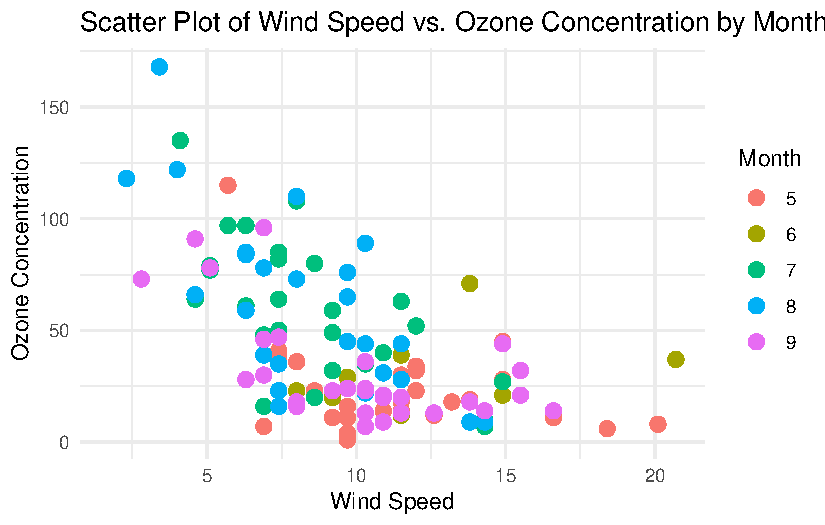
\includegraphics{InClass2_files/figure-pdf/unnamed-chunk-2-1.pdf}

}

\end{figure}

\begin{Shaded}
\begin{Highlighting}[]
\FunctionTok{ggplot}\NormalTok{(airquality, }\FunctionTok{aes}\NormalTok{(}\AttributeTok{x =} \FunctionTok{factor}\NormalTok{(Month), }\AttributeTok{y =}\NormalTok{ Ozone, }\AttributeTok{fill =} \FunctionTok{factor}\NormalTok{(Month))) }\SpecialCharTok{+}
  \FunctionTok{geom\_bar}\NormalTok{(}\AttributeTok{stat =} \StringTok{"summary"}\NormalTok{, }\AttributeTok{fun =} \StringTok{"mean"}\NormalTok{, }\AttributeTok{position =} \StringTok{"dodge"}\NormalTok{, }\AttributeTok{color =} \StringTok{"black"}\NormalTok{) }\SpecialCharTok{+}
  \FunctionTok{labs}\NormalTok{(}\AttributeTok{title =} \StringTok{"Average Ozone Concentration by Month"}\NormalTok{,}
       \AttributeTok{x =} \StringTok{"Month"}\NormalTok{,}
       \AttributeTok{y =} \StringTok{"Average Ozone Concentration"}\NormalTok{) }\SpecialCharTok{+}
  \FunctionTok{theme\_minimal}\NormalTok{()}
\end{Highlighting}
\end{Shaded}

\begin{verbatim}
Warning: Removed 37 rows containing non-finite values (`stat_summary()`).
\end{verbatim}

\begin{figure}[H]

{\centering 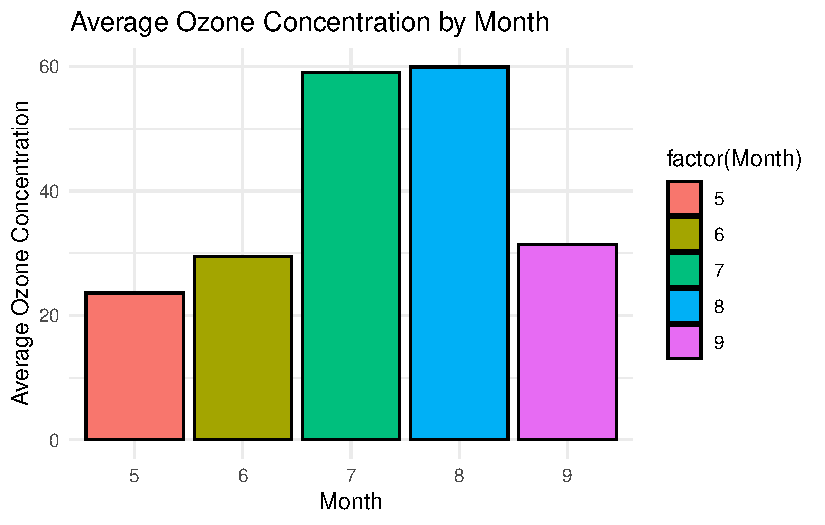
\includegraphics{InClass2_files/figure-pdf/unnamed-chunk-3-1.pdf}

}

\end{figure}

\bookmarksetup{startatroot}

\hypertarget{shiny-app}{%
\chapter{Shiny App}\label{shiny-app}}

\#\# \textbf{Shiny Application about Air Quality}

\#\# \textbf{Link to Shinyapps.io}

\href{https://ozgenursensoy.shinyapps.io/ShinyApp/}{My Shiny App}

\bookmarksetup{startatroot}

\hypertarget{operations_research}{%
\chapter{Operations\_Research}\label{operations_research}}

\bookmarksetup{startatroot}

\hypertarget{easyparks-parking-optimization-with-gurobi}{%
\chapter{EasyPark's Parking Optimization with
Gurobi}\label{easyparks-parking-optimization-with-gurobi}}

\textbf{Business Context}

EasyPark tackles urban traffic congestion and driver frustration by
optimizing parking. With 30\% of city vehicles searching for parking,
EasyPark enhances the urban parking experience using mathematical
optimization.

\textbf{Problem}

Cruising for parking worsens congestion, wastes time and fuel, and
increases carbon emissions. Traditional parking methods fail to address
drivers' challenges, causing delays and urban gridlock.

\textbf{Solution}

EasyPark's innovative solution involves a mathematical optimization
model powered by Gurobi, focusing on real-time data inputs to
efficiently guide users to available parking spots.

\textbf{How It Works}

\emph{Data Collection:} EasyPark uses machine learning for comprehensive
data, including historical transactions, mapping, GIS, user
transactions, and routes.

\emph{Probability Estimation:} Bayesian models estimate the probability
of finding parking by time and city block using collected data.

\emph{Mixed-Integer Programming (MIP):} EasyPark employs an MIP model to
find the best route, minimizing travel time based on the user's
destination and spot probabilities.

\textbf{Personal Commentary}

EasyPark's innovative approach not only reduces parking search time but
also promotes a sustainable urban lifestyle. Using advanced technology
like Gurobi, it showcases smart solutions in urban planning, impacting
individual convenience with dynamic pricing and aiding in optimal
capacity planning. This solution acts as a catalyst, enhancing city
life, improving traffic flow, and meeting the demands of modern urban
living.

\textbf{Reference}

\href{https://www.gurobi.com/case_studies/easy-park-urban-parking-optimization/}{\emph{https://www.gurobi.com/case\_studies/easy-park-urban-parking-optimization/}}

\bookmarksetup{startatroot}

\hypertarget{part-1}{%
\chapter{\texorpdfstring{\textbf{Part 1}}{Part 1}}\label{part-1}}

\textbf{Final}

\textbf{Özgenur Şensoy}

\textbf{08.01.2024}

\textbf{Q1}

AI regulation requires a delicate balance. Overly strict rules hinder
innovation, while a lack of regulations risks chaos. High-risk areas
like medical diagnosis face stringent scrutiny, ensuring citizen
protection, while low-risk applications have lighter burdens, fostering
progress. Though incumbents may benefit from navigating complex
regulations, startups can thrive in less-regulated spaces. Effective
regulations address ethical concerns and prevent misuse, creating a
level playing field. Encouraging transparency, open-source AI, and
investing in AI literacy further empower users and developers. While
embracing ambiguity initially, a comprehensive approach ensures a
sustainable, inclusive AI future by building trust, promoting
collaboration, and attracting investment.

\textbf{Q2}

1- Define Scope and Stakeholders: Clearly outline project boundaries and
gather stakeholder expectations.

2- Understand Current Process: Gather requirements by interviewing team
members and observing the manual process.

3- Data Collection, Cleaning, and EDA: Collect and clean relevant data
from Excel sheets, and perform exploratory data analysis.

4- Define Metrics and Model Development: Establish key performance
indicators, select technology, and develop a prototype for automation.

5- Iteration, Testing, and Feedback: Iterate on the solution, thoroughly
test, and gather feedback for improvements.

6- Documentation, Training, and Implementation: Document the process,
train the team, and gradually implement the automated solution.

7- Monitoring, Maintenance, and Optimization: Set up monitoring, address
issues, and establish a maintenance plan. Continuously optimize based on
user feedback.

8- Scale and Review: Consider scaling the solution, update
documentation, and conduct a post-implementation review for lessons
learned.

\textbf{Q3}

\begin{Shaded}
\begin{Highlighting}[]
\FunctionTok{library}\NormalTok{(dslabs)}
\FunctionTok{library}\NormalTok{(ggplot2)}

\NormalTok{results\_us\_election\_2016}\SpecialCharTok{$}\NormalTok{clinton\_percent }\OtherTok{\textless{}{-}}\NormalTok{ results\_us\_election\_2016}\SpecialCharTok{$}\NormalTok{clinton }\SpecialCharTok{/} \DecValTok{100}
\NormalTok{results\_us\_election\_2016}\SpecialCharTok{$}\NormalTok{trump\_percent }\OtherTok{\textless{}{-}}\NormalTok{ results\_us\_election\_2016}\SpecialCharTok{$}\NormalTok{trump }\SpecialCharTok{/} \DecValTok{100}
\NormalTok{results\_us\_election\_2016}\SpecialCharTok{$}\NormalTok{others\_percent }\OtherTok{\textless{}{-}}\NormalTok{ results\_us\_election\_2016}\SpecialCharTok{$}\NormalTok{others }\SpecialCharTok{/} \DecValTok{100}


\FunctionTok{set.seed}\NormalTok{(}\DecValTok{42}\NormalTok{)  }\CommentTok{\# Set seed for reproducibility}
\NormalTok{random\_states }\OtherTok{\textless{}{-}} \FunctionTok{sample}\NormalTok{(results\_us\_election\_2016}\SpecialCharTok{$}\NormalTok{state, }\DecValTok{20}\NormalTok{)}

\NormalTok{df }\OtherTok{\textless{}{-}}\NormalTok{ results\_us\_election\_2016[results\_us\_election\_2016}\SpecialCharTok{$}\NormalTok{state }\SpecialCharTok{\%in\%}\NormalTok{ random\_states, ]}

\NormalTok{df\_melted }\OtherTok{\textless{}{-}}\NormalTok{ reshape2}\SpecialCharTok{::}\FunctionTok{melt}\NormalTok{(df, }\AttributeTok{id.vars =} \FunctionTok{c}\NormalTok{(}\StringTok{"state"}\NormalTok{, }\StringTok{"electoral\_votes"}\NormalTok{))}

\FunctionTok{ggplot}\NormalTok{(df\_melted, }\FunctionTok{aes}\NormalTok{(}\AttributeTok{x =}\NormalTok{ state, }\AttributeTok{y =}\NormalTok{ value, }\AttributeTok{fill =}\NormalTok{ variable)) }\SpecialCharTok{+}
  \FunctionTok{geom\_bar}\NormalTok{(}\AttributeTok{stat =} \StringTok{"identity"}\NormalTok{, }\AttributeTok{position =} \StringTok{"stack"}\NormalTok{) }\SpecialCharTok{+}
  \FunctionTok{labs}\NormalTok{(}\AttributeTok{title =} \StringTok{"2016 US Election Results in 20 Randomly Selected States"}\NormalTok{,}
       \AttributeTok{x =} \StringTok{"State"}\NormalTok{,}
       \AttributeTok{y =} \StringTok{"Percentage of Votes"}\NormalTok{) }\SpecialCharTok{+}
  \FunctionTok{scale\_y\_continuous}\NormalTok{(}\AttributeTok{labels =}\NormalTok{ scales}\SpecialCharTok{::}\FunctionTok{percent\_format}\NormalTok{(}\AttributeTok{scale =} \DecValTok{1}\NormalTok{)) }\SpecialCharTok{+}
  \FunctionTok{theme}\NormalTok{(}\AttributeTok{axis.text.x =} \FunctionTok{element\_text}\NormalTok{(}\AttributeTok{angle =} \DecValTok{45}\NormalTok{, }\AttributeTok{hjust =} \DecValTok{1}\NormalTok{)) }\SpecialCharTok{+}
  \FunctionTok{scale\_x\_discrete}\NormalTok{(}\AttributeTok{limits =}\NormalTok{ random\_states)  }\CommentTok{\# Set x{-}axis limits to the 20 random states}
\end{Highlighting}
\end{Shaded}

\begin{figure}[H]

{\centering 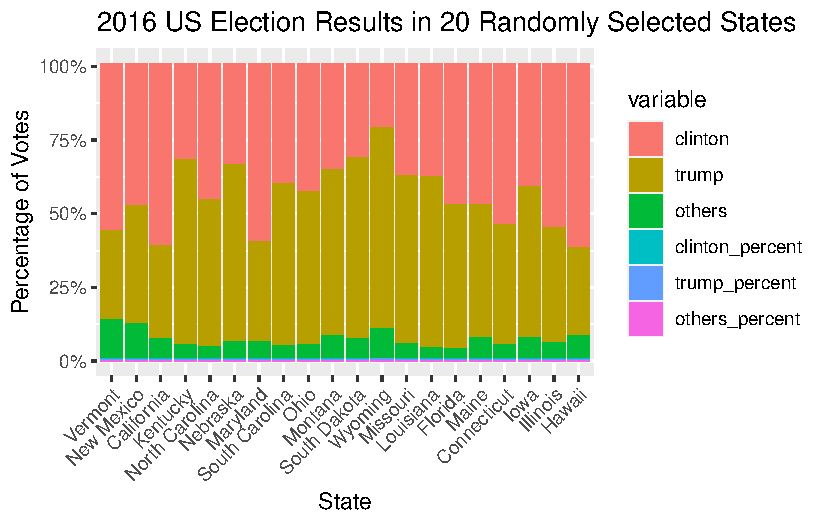
\includegraphics{Final_files/figure-pdf/unnamed-chunk-1-1.pdf}

}

\end{figure}

Given the existing code and the context of the dataset, a suitable graph
to visualize the 2016 US election results in 20 randomly selected states
would be a grouped bar plot representing the percentage of votes for
each candidate (Clinton, Trump, and Others) in each state. This type of
graph allows for a clear comparison of vote percentages across
candidates within each state. (Randomly selected states may be
representative of geographic and demographic differences. Therefore, by
focusing on the election results in these states, we can better
understand the political trends of a particular region or region. Of
course, we can do it by adding all the states.)

A grouped bar plot is chosen because it allows for a straightforward
comparison of the percentage of votes for each candidate within each
state. Each bar represents a state, and the bars are grouped by
candidate, making it easy to observe the variations in vote percentages
across states. The output will be a grouped bar plot with bars for each
state, showing the percentage of votes for Clinton, Trump, and Others,
providing a clear visual comparison.

\bookmarksetup{startatroot}

\hypertarget{part-2}{%
\chapter{\texorpdfstring{\textbf{Part 2}}{Part 2}}\label{part-2}}

SC184*** mean math score, mean read score and mean sci score ``Does your
school offer professional development to \# science teachers in any of
the following? \#pisa\$SC184Q01JA \# 1Yes 2No \# set 1 as yes and 2 as
no

pisa\_SC184Q01JA \textless- pisa \%\textgreater\% mutate(SC184Q01JA =
ifelse(SC184Q01JA == 1, ``Yes'', ``No'')) \# drp the NA

pisa\_SC184Q01JA \textless- pisa\_SC184Q01JA \%\textgreater\%
filter(!is.na(SC184Q01JA))

professional\_development\_to\_science\_teachers \textless-
pisa\_SC184Q01JA \%\textgreater\% group\_by(SC184Q01JA) \%\textgreater\%

summarise(mean\_sci = mean(mean\_sci, na.rm = TRUE))

\bookmarksetup{startatroot}

\hypertarget{line-plot-normalize-the-data}{%
\chapter{line plot normalize the
data}\label{line-plot-normalize-the-data}}

ggplot(professional\_development\_to\_science\_teachers, aes(x =
SC184Q01JA, y = mean\_sci)) + geom\_bar(stat = ``identity'', fill =
``\#dda0dd'') + labs(title = ``Mean Science Score by Professional
Development to Science Teachers'',

\begin{verbatim}
     x = "Professional Development to Science Teachers",
     y = "Mean Sci Score") +
     
theme_bw() +
theme(plot.title = element_text(hjust = 0.5))
\end{verbatim}

\begin{Shaded}
\begin{Highlighting}[]

\end{Highlighting}
\end{Shaded}

When we checked for math, we obtained more distant bars. However, when I
checked for science, I noticed that the bars were closer.

Supporting the impact of professional development argues that
well-designed programs can enhance teachers' content knowledge,
instructional strategies, and classroom management skills. These
improvements, in turn, are expected to positively influence student
engagement, understanding, and achievement in science. Investing in
ongoing teacher development contributes to a more dynamic and effective
learning environment.

In conclusion, the relationship between professional development for
teachers and students' science performance is multifaceted and nuanced.
While some argue for the positive impact of well-implemented programs on
teacher effectiveness and subsequently on student outcomes, others
highlight the need for a more tailored and context-specific approach to
professional development. Further research and exploration into the
specific elements that contribute to the success or lack thereof in
science education are essential to provide more conclusive insights into
this complex relationship.



\end{document}
